\documentclass{report}

\usepackage[utf8]{inputenc}
\usepackage[nottoc]{tocbibind}
\usepackage{vhistory}
\usepackage[ampersand]{easylist}
\usepackage{natbib}
\usepackage{url}
\usepackage{scrextend}
\usepackage{graphicx}
\usepackage{multicol}
\usepackage[titletoc]{appendix}
\usepackage{float}
\usepackage{blindtext}
\usepackage{listings}
\usepackage{xcolor}
\usepackage{tabto} \NumTabs{3}

\lstdefinelanguage{alloy} {
	morekeywords={assert, pred, all, no, lone, one, some, check, run, but, let, implies, not, iff, in, and, or, set, sig, Int, int, if, then, else, exactly, disj, fact, fun, module, abstract, extends, open, none, univ, iden, seq,},
	sensitive=false,
	morecomment=[l]{//},
	morecomment=[s]{/*}{*/},
	morestring=[b]", }

\definecolor{alloyBlue}{HTML}{2d38b0}
\definecolor{alloyGreen}{HTML}{00a130}

\lstset{
	basicstyle=\small,
	keywordstyle=\color{alloyBlue}\bfseries,
	identifierstyle=,
	commentstyle=\color{alloyGreen},
	stringstyle=\ttfamily,
	showstringspaces=false,
	tabsize=4,
}

\graphicspath{ {img/} }

\begin{document}

\begin{titlepage}
	\centering
	
\includegraphics[width=0.5\textwidth]{polimi-logo}\par\vspace{1cm}
	{\scshape\LARGE Politecnico di Milano\par}
	\vspace{1cm}
	{\scshape\Large Software Engineering 2 project\par}
	\vspace{1.5cm}
	{\huge\bfseries PowerEnJoy\par}
	\vspace{2cm}
	\begin{multicols}{2}
		{\Large\itshape Matteo Penco\par}
		\vspace{0.25cm}
		mat. 875740
		\vfill\columnbreak
		{\Large\itshape Riccardo Pressiani\par}
		\vspace{0.25cm}
		mat. 874948
	\end{multicols}
	
	\vfill
	
	{\Large Version 0.1 draft\par}
	\vspace{1.25cm}
	{\large \today\par}
\end{titlepage}

\begin{versionhistory}
  \vhEntry{0.1}{26.10.16}{RP}{Document created}
\end{versionhistory}

\vspace{5cm}
{\noindent\Huge\bfseries Hours of work\par}
\vspace{0.5cm}
{\noindent Matteo Penco	\tab{35h}\par}
{\noindent Riccardo Pressiani \tab{35h}\par}

\tableofcontents

%Introduction
\chapter{Introduction}
This section introduces the Requirements Analysis and Specification Document for the PowerEnJoy platform to its readers.

\section{Purpose}
\section{Scope}
\section{Definitions, acronyms and abbreviations}

\subsection{Definitions}
	\begin{labeling}{defs}
		\item[\textbf{Onboard computer}] An onboard computer is intend to be the embedded device integrated in the car system that provide two main functions: on one hand it shows the user basic information about the ongoing rent, on the other hand it is in charge of all the communications related to the state of the car between the car and the PowerEnJoy management system.
		\item[\textbf{Safe area}] A safe area is an area, within predefined edges, in which the users are allowed to park the rented cars. The users is not allowed to park, and therefore end a rent, if he/she is not inside a safe area.
	\end{labeling}
\subsection{Acronyms}
	\begin{labeling}{acro}
		\item[\textbf{GPS}] Global Positioning System
		\item[\textbf{PIN}] Personal Identification Number
	\end{labeling}
\subsection{Abbreviations}
	% \begin{labeling}{abbrv}
	% 	\item[\textbf{ABBRV1}] abbrv1
	% \end{labeling}
\section{References}
\section{Overview}

%Overall Description
\chapter{Overall Description}

\section{Product perspective}
\section{Product functions}

\begin{labeling}{main-funcs}
	\item[\textbf{Registration}] The system allows and requires the user to register before accessing the services of the app. In this phase the user uploads his/her ID document and driver licence and provides the credential for his/her preferred payment method.
	\item[\textbf{Map exploration}] The system allows the user to explore a map and to look for available cars near either his/her location or a given address.
	\item[\textbf{Car reservation}] The system allows the user to reserve a car for a limited amount of time. During this interval the car is parked but cannot be reserved or rented by any other user of the PowerEnJoy platform.
	\item[\textbf{Car rental}] The system allows the user to rent a car that he/she has previously reserved. The rental starts once the user ignites the engine of the car. The cost of the service is determined by the duration of the rental.
\end{labeling}
\section{User characteristics}
\section{Constraints}
\subsection{Regulatory polices}
During the registration phase the user is required to allow PowerEnJoy to manage the sensible data he/she is providing. Moreover, the user need to allow the system to access his current location in order to use the services provided by the platform. All the issues related to the user privacy must follow the state regulations.

\subsection{Hardware limitations}
\begin{itemize}
	\item The user must have access to an Internet connection in order to reserve a car from the web app or the mobile app.
	\item The user must activate the GPS module and have access to a data connection on one of its devices in order to unlock the car once he/she has reached it.
	\item The GPS receiver equipped in the cars must be always active in order to communicate the car location to the system.
	\item All the cars must have an active data connection in order to communicate and receive the necessary information from the system.
\end{itemize}

\subsection{Interfaces to other applications}
The system needs to integrate an external service for the menagement of the payment methods. All the major payment methods must be supported by the application, including the most popular credit card circuits (including Visa, MasterCard and American Express) and PayPal.
\section{Assumptions and dependencies}

\begin{itemize}
	\item In order to register, the user must insert his/her credentials, including identity card and driving license.
	\item The system submits in the database the user registered matched with the provided PIN.
	\item Every car is equipped with a sensor that communicates to the system if the car's engine is running or not. The value of this sensor is ON for the former case, OFF for the latter.
	\item Every car is equipped with an onboard computer.
	\item Every car is equipped with a GPS receiver that communicates the car location to the system. The data transmitted to the system corresponds to the geographic coordinates of the car location.
	\item The system can automatically lock and unlock the car.
	\item The car's seats are equipped with a sensor able to detect the presence of a person seated in the car. The signal transmitted to the system is equal to 1 if a person is detected, 0 (zero) otherwise.
	\item The car can inform the system whether the doors are closed or not. If at least one of the door is open, the value transimitted is equal to 0 (zero), 1 otherwise.
	\item The set of safe areas is pre-defined by the system.
	\item The set of safe areas provided with power grid stations is pre-defined by the system.
	\item The car can inform the system about the battery level. The value transmitted is equal to the percentage of the battery charge available. Moreover, the car communicates to the system if the battery is charging or not.
	\item An external service is integrated in the system in order to manage billing operations.
\end{itemize}
%Specific requirements
\chapter{Specific Requirements}
This chapter provides a high detaild description of both functional and non functional software requirements.

%\section{External interface requirements}
\section{Functional requirements}

\subsection{Goal 1}
User is able to register in the system.

\setcounter{secnumdepth}{3}
\subsubsection{Functional requirement 1.1}
If credentials and payment information given by the user are valid and he is not present in the database as an already registered user, then the new user is registered and submitted in the database.

\subsection{Goal 2}
Users registered receive a PIN to insert in the reserved car's onboard computer in order to drive it.

\setcounter{secnumdepth}{3}
\subsubsection{Functional requirement 2.1}
If user's registration succeeds, then the system generates a new PIN for the registered user and communicates it via mail.
\subsection{Goal 3}
User is able to log in the system.

\setcounter{secnumdepth}{3}
\subsubsection{Functional requirement 3.1}
If the user inserts correct credentials and password, then the system allows the user to log in.

\subsection{Goal 4}
The user is able to find the location of all the available cars near is current position or near a specified address.

\setcounter{secnumdepth}{3}
\subsubsection{Functional requirement 4.1}
If the user has his GPS activated and there are available cars near his position or near the specified address, then the system shows onto the web app the position of these cars.

\subsection{Goal 5}
User is able to book a car for up to an hour before picking it up.

\setcounter{secnumdepth}{3}
\subsubsection{Functional requirement 5.1}
If the user is logged, has no ongoing booking or rental and the car selected is AVAILABLE, then the user can book the car. The system creates a booking related to that user and that car.

\subsubsection{Functional requirement 5.2}
The system tags the car as RESERVED.

\subsection{Goal 6}
User is able to check the battery level of a car before booking it.

\setcounter{secnumdepth}{3}
\subsubsection{Functional requirement 6.1}
If the user chooses a car to book then, before confirming the booking, the system shows the battery level of the car chosen.\\~\\
\noindent Domain assumptions required: [A13]
\subsection{Goal 7}

\setcounter{secnumdepth}{3}
\subsubsection{Functional requirement 7.1}

\subsubsection{Functional requirement 7.2}

\subsubsection{Functional requirement 7.3}

\subsection{Goal 8}
If a car is not picked up within one hour from the booking the reservation expires and the user pays a fee of 1 EUR.

\setcounter{secnumdepth}{3}
\subsubsection{Functional requirement 8.1}
When the user books a car, a stopwatch starts: if one hour has passed and no rental, related to that booking, has been created, then the booking expires.\\~\\
\noindent Domain assumptions required: [A15]

\subsubsection{Functional requirement 8.2}
 the system tags the car as AVAILABLE.

\subsubsection{Functional requirement 8.3}
 If the booking has expired, the system charges the user a fee of 1 EUR.
\subsection{Goal 8}
User is able to open the reserved car.

\setcounter{secnumdepth}{3}
\subsubsection{Functional requirement 8.1}
If the comparison, through GPS systems, between positions of the user and the reserved car indicates that the user reached the "opening distance", then the user can tell to the system to open the reserved car.
\subsection{Goal 10}
The user can start a rental by inserting his/her PIN and then by igniting the engine.

\setcounter{secnumdepth}{3}
\subsubsection{Functional requirement 10.1}
Once the user has entered his/her PIN, if the system confirms that it is correct, the user is allowed to ignite the engine.\\~\\
\noindent Domain assumptions required: [A6, A7]

\subsubsection{Functional requirement 10.2}
If the engine is set to ON, the system creates a rental related to the user's ongoing booking and a stopwatch starts in order to measure the time elapsed from the begin of the rental.\\~\\
\noindent Domain assumptions required: [A3]

\subsubsection{Functional requirement 10.3}
The system calculates the current cost of the rental by multiplying the minutes elapsed by a fixed rate per minute.\\~\\
\noindent Domain assumptions required: [A12]

\subsubsection{Functional requirement 10.4}
When the rental begins, the system tags the car as IN USE.

\subsection{Goal 11}
If the user leaves a car with the battery level higher than 50\%, he/she is eligible for a 20\% discount on the last ride.

\setcounter{secnumdepth}{3}
\subsubsection{Functional requirement 11.1}
If the user ends a rental leaving the car with the battery level higher than 50\%, the system applies a 20\% discount on the total cost of the last rental.

\subsection{Goal 12}
The rental ends when the user parks in a safe area and exit the car.

\setcounter{secnumdepth}{3}
\subsubsection{Functional requirement 12.1}
If the engine is set to OFF, the GPS location of the car is whitin one of the safe areas defined by the system administrator, the seat sensors are all set to 0 (zero) and all the car's doors are closed the rental ends.

\subsubsection{Functional requirement 12.2}
If the rental is ended the related watchstop stops and the final cost of the fare is calculated by the system.

\subsubsection{Functional requirement 12.3}
If the user is no eligible for additional discount or penalities on the final cost of the rental, the user is billed according to the payment method that he/she has provided.

\subsubsection{Functional requirement 12.4}
The car related to an ended rental is set from IN USE to AVAILABLE.

\subsection{Goal 13}
If the user shares the rented car with at least two passengers during the whole duration of the rental, he/she is eligible for a 10\% discount on the total cost of that rental.

\setcounter{secnumdepth}{3}
\subsubsection{Functional requirement 13.1}
If at least three seat sensors are set to 1 from the moment the engine is set to ON to the moment it is set to OFF, the system applies a 10\% discount on the total cost of the last rental.\\~\\
\noindent Domain assumptions required: [A3, A8]
\subsection{Goal 14}
If the user leaves a car with the battery level higher than 50\%, he/she is eligible for a 20\% discount on the last ride.

\setcounter{secnumdepth}{3}
\subsubsection{Functional requirement 14.1}
If the user ends a rental leaving the car with the battery level higher than 50\%, the system applies a 20\% discount on the total cost of the last rental.\\~\\
\noindent Domain assumptions required: [A13]

\subsection{Goal 15}
If the car is left within one of the special parking areas and the user takes care of plugging the car into the power grid, he/she is eligible for a 30\% discount on the last ride.

\setcounter{secnumdepth}{3}
\subsubsection{Functional requirement 15.1}
If the rental is ended, the GPS location of the car is whitin one of the special parking areas and the battery is charging, the system applies a 30\% discount on the total cost of the last rental.

\subsubsection{Functional requirement 15.2}
In order to apply the discount, the car has to be plugged to the power grid within a minute after the rental is ended.

\subsection{Goal 16}
If the car is left at more than 3KM from the nearest specia parking area or with the battery charge lower than 20\%, the user will pay an extra fee that will correspond to the 30\% of the cost of the last ride.

\setcounter{secnumdepth}{3}
\subsubsection{Functional requirement 16.1}
The system charges the user 30\% more on the total cost of the last ride if at least one of the following condition is verified:
\begin{itemize}
	\item The rental is ended and the distance between the GPS coordinates of the car and the ones of the nearest special parking area is more than 3KM.
	\item The rental is ended and the battery level is lower than 20\%.
\end{itemize}

\noindent Domain assumptions required: [A5, A11, A13]

\section{Performance requirements}
%\section{Design constraints}
\section{Software system attributes}
%\section{Other requirements}


\begin{appendices}
	%Scenarios and UML models
	\chapter{Scenarios and UML models}

\section{Scenarios}
\blindtext

\subsection{Scenario 1}
\blindtext

\subsection{Scenario 2}
\blindtext

\subsection{Scenario 3}
\blindtext

\section{Use case diagram}

\subsection{Use case description 1}
\subsection{Use case description 2}
\subsection{Use case description 3}
\section{State diagrams}

\begin{figure}[H]
	\centering
	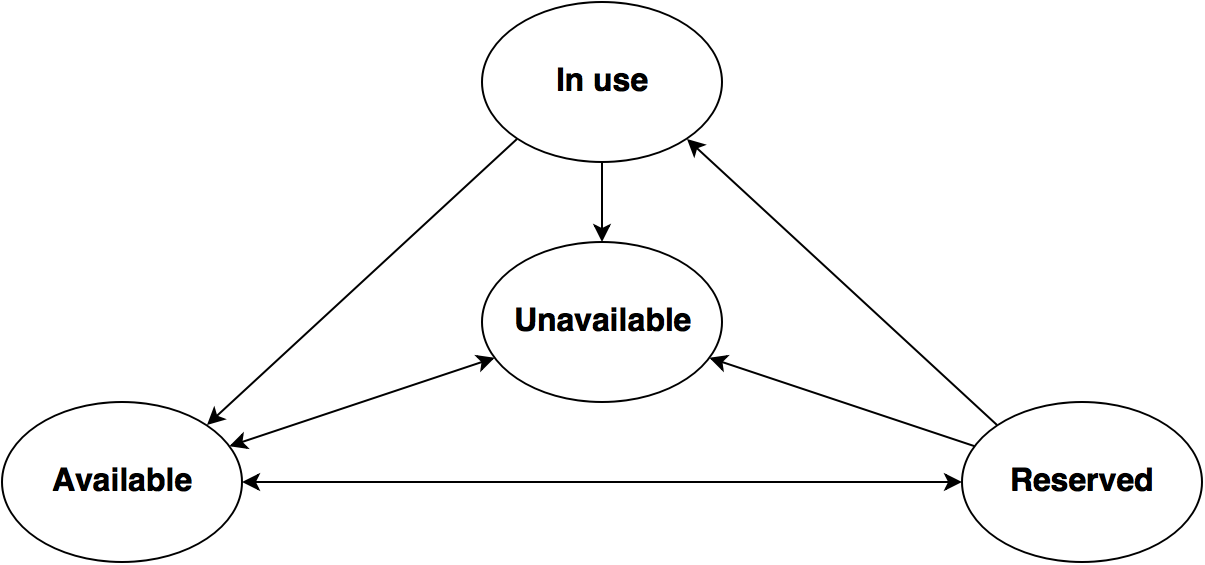
\includegraphics[width=\textwidth]{car-state-diagram}
	\caption[Car state diagram]{This state diagram represent the possible transitions among the car states.}
	\label{fig:car-state-diagram}
\end{figure}
\newpage
\section{Class diagram}

\begin{figure}[H]
	\centering
	\includegraphics[width=1.45\textwidth, angle=90]{class-diagram}
	\caption[Class diagram]{This diagram represents the class structure of PowerEnJoy system.}
	\label{fig:class-diagram}
\end{figure}

	%Alloy
	\chapter{Alloy modelling}
\end{appendices}

\listoffigures
\begingroup
\let\clearpage\relax
%\listoftables
\endgroup

\bibliographystyle{unsrt}
\bibliography{ref}

\end{document}
